% ============================================================================
% Panel captions for the causal-knowledge-graph runtime paper.
% Five result panels, each four charts wide with a leading 3D chart.
% Every number below is read from validation/results/*.json; the panels are
% produced by validation/make_panels.py.
% Copy any block into the manuscript, or \input this file where the panels
% should appear.
% ============================================================================

% ---------------------------------------------------------------------------
% Panel 1: trajectory emergence  (Thm. emergence, Prop. no-edges)
% ---------------------------------------------------------------------------
\begin{figure*}[!htbp]
    \centering
    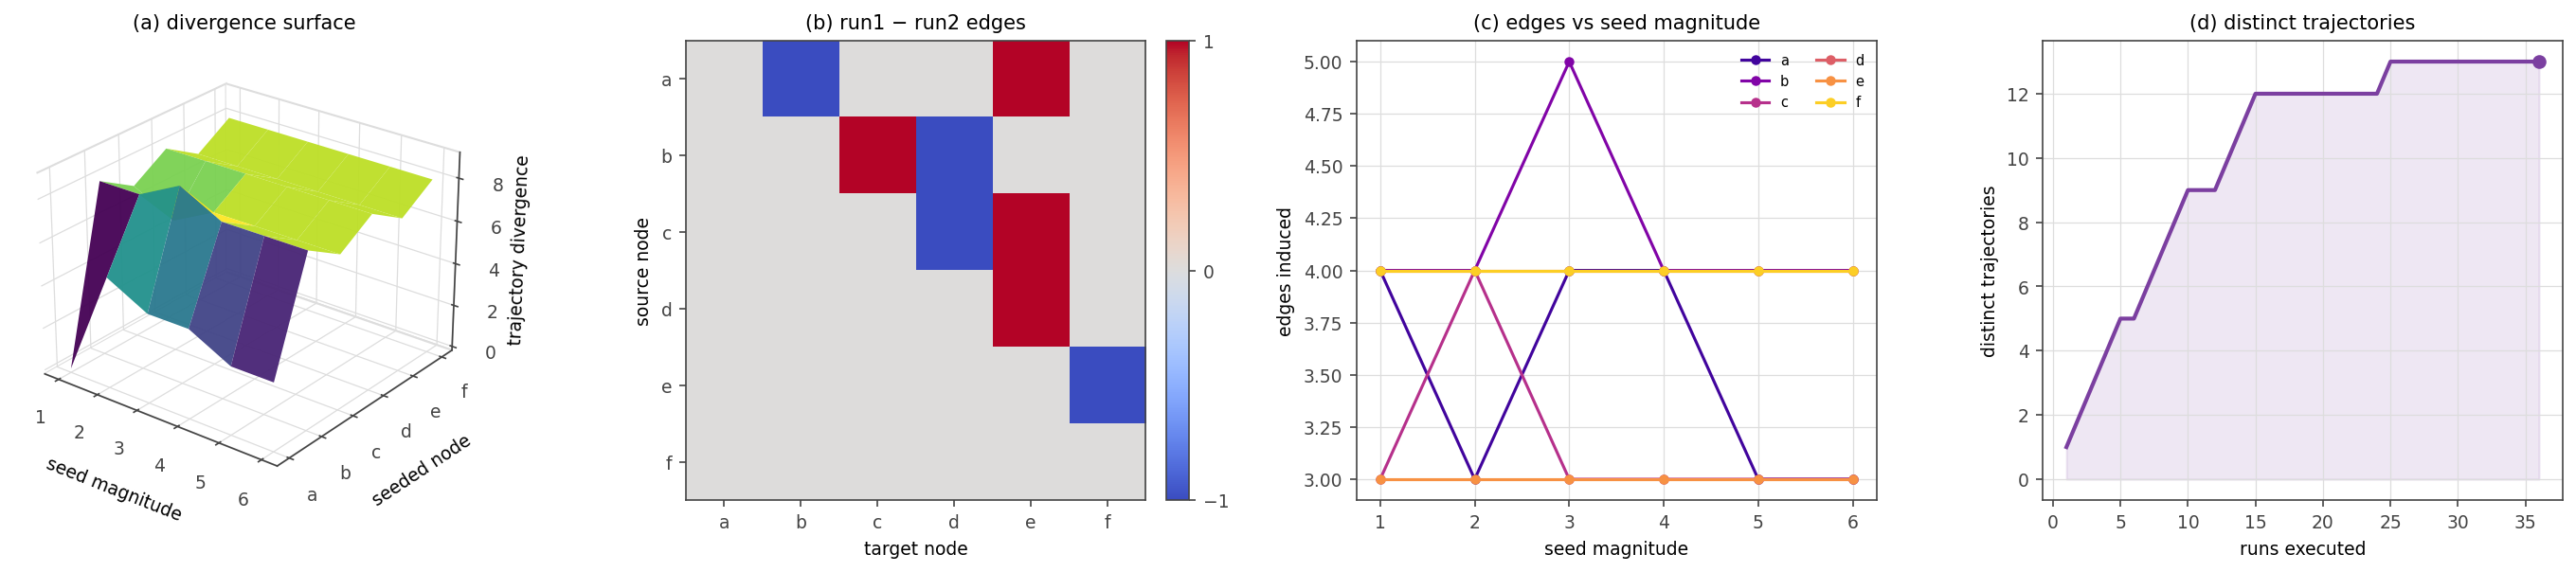
\includegraphics[width=\textwidth]{figures/panel_trajectory.png}
    \caption{\textbf{The Trajectory is Induced by the Run, Not Scheduled Before It.}
    Executable model (\texttt{validation/trajectory\_emergence.py}) over one fixed
    six-node catalogue $\{a,b,c,d,e,f\}$; each run seeds a single node and lets a
    carrier module propagate signal a distance equal to the run-produced value.
    (\textbf{A})~Three-dimensional viridis surface of trajectory divergence---edges
    differing from the quiet baseline---over seeded node (six-valued $y$-axis,
    $a$ through $f$) and seed magnitude (linear $x$-axis, $1$ to $6$), viewing angle
    elevation $26^{\circ}$ azimuth $-52^{\circ}$. Divergence spans $0$ to $9$ edges:
    a single run-time value at a single node reshapes the entire causal edge
    relation. This is the empirical content of Theorem~\ref{thm:emergence}
    (Trajectory Emergence): the induced relation is a function of values produced
    only during the run.
    (\textbf{B})~Signed difference heat map (coolwarm, range $[-1,1]$) of the two
    induced adjacency matrices, source node on the $y$-axis versus target node on
    the $x$-axis over the ordered set $a$--$f$. Seeding node $a$ induces
    $\{a\!\to\!e,\,b\!\to\!c,\,c\!\to\!e,\,d\!\to\!e\}$; seeding node $d$ induces
    $\{a\!\to\!b,\,b\!\to\!d,\,c\!\to\!d,\,e\!\to\!f\}$. Red cells are edges present
    only in the first run, blue only in the second; the eight-edge symmetric
    difference is non-empty, so no single fixed edge set equals both.
    (\textbf{C})~Edges induced (linear $y$-axis) versus seed magnitude (linear
    $x$-axis, $1$ to $6$), one plasma-coloured line per seeded node. The edge count
    ranges from $3$ to $5$ and moves non-monotonically with the seeded value,
    node by node---which reads occur is decided in-run
    (Proposition~\ref{prop:no-edges}).
    (\textbf{D})~Cumulative distinct trajectories (linear $y$-axis) against runs
    executed (linear $x$-axis, $1$ to $36$), purple curve with shaded fill. Over the
    same node set, $36$ runs discover $13$ distinct trajectories; the discovery
    curve rises steeply and saturates, marking the run-constituted trajectory as
    visibly multivalued rather than schedulable.}
    \label{fig:panel-trajectory}
\end{figure*}

% ---------------------------------------------------------------------------
% Panel 2: run to completion vs halt-on-error  (Thm. no-exit, Cor. completion, Def. exec)
% ---------------------------------------------------------------------------
\begin{figure*}[!htbp]
    \centering
    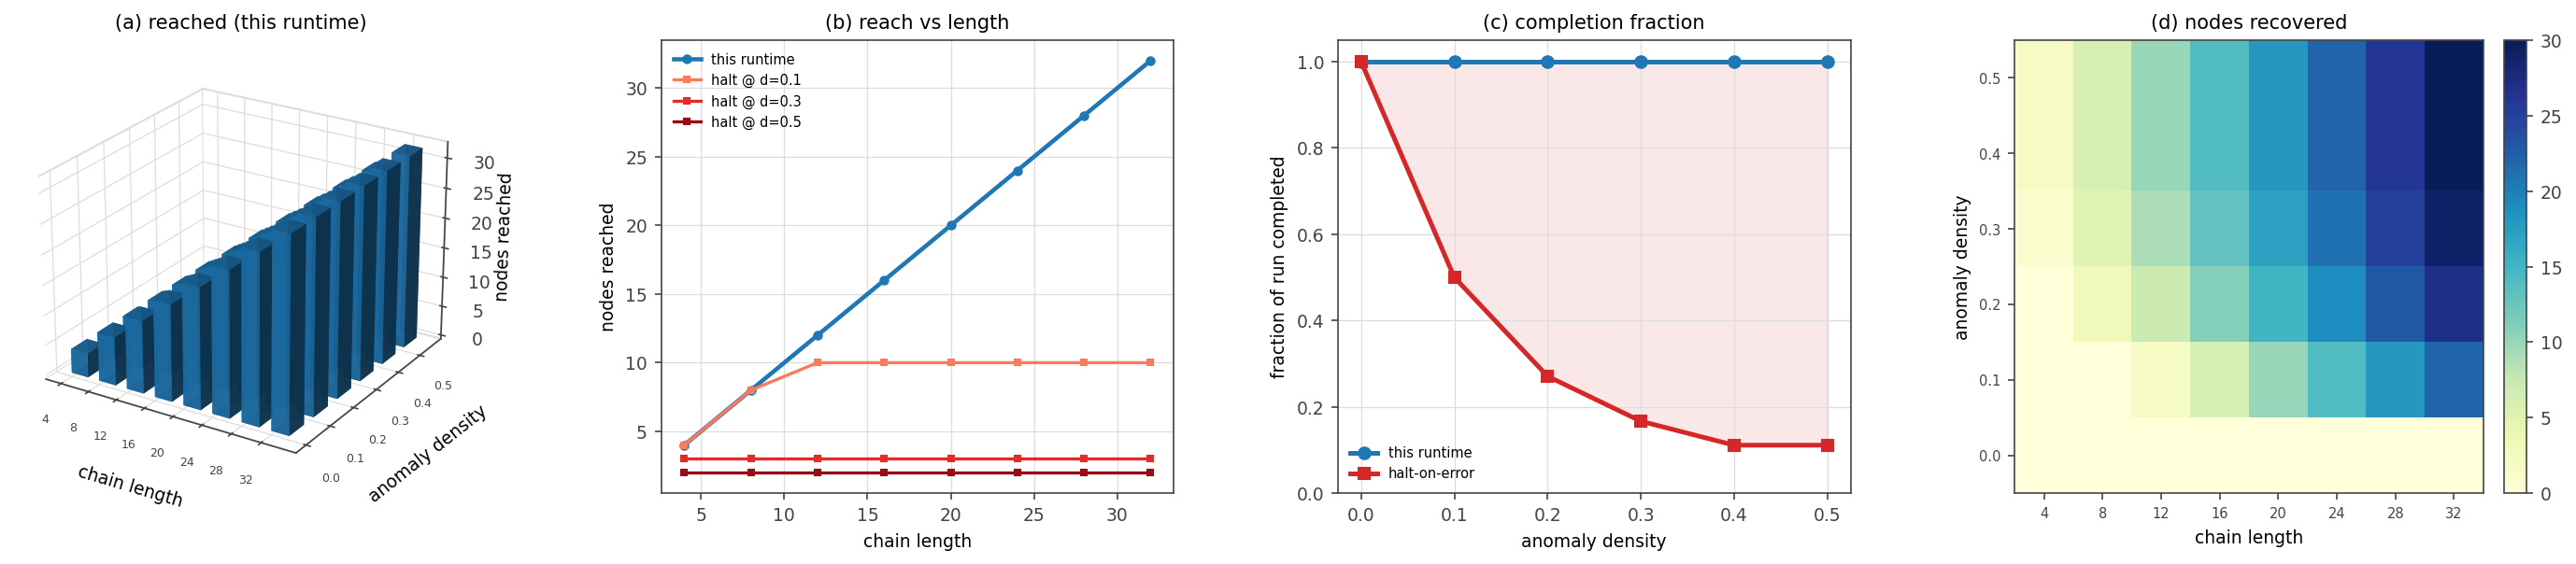
\includegraphics[width=\textwidth]{figures/panel_completion.png}
    \caption{\textbf{Run to Completion Versus Halt on Error.}
    Executable model (\texttt{validation/run\_to\_completion.py}) sweeping linear
    chains of length $L \in \{4,8,\dots,32\}$ against anomaly density
    $d \in \{0.0,0.1,\dots,0.5\}$; at each density a deterministic fraction of nodes
    carry a chunk that raises.
    (\textbf{A})~Three-dimensional steel-blue bar field of nodes reached by this
    runtime over chain length ($x$-axis, $4$ to $32$) and anomaly density
    ($y$-axis, $0.0$ to $0.5$), viewing angle elevation $24^{\circ}$ azimuth
    $-58^{\circ}$. The bars form a full plane: every one of the $L$ nodes executes
    in every cell of the $8 \times 6$ sweep, independent of how many chunks raise.
    This is the empirical content of Corollary~\ref{cor:completion}
    (Run to Completion): a raising chunk does not halt the run.
    (\textbf{B})~Nodes reached (linear $y$-axis) versus chain length (linear
    $x$-axis, $4$ to $32$). The steel-blue line for this runtime tracks the diagonal
    ($L$ nodes reached for every $L$); the red halt-on-error lines
    (densities $0.1$, $0.3$, $0.5$) plateau at the first anomaly---at
    $d=0.5$ the halt-on-error runtime reaches only $2$ nodes regardless of chain
    length.
    (\textbf{C})~Fraction of the run completed (linear $y$-axis, $0$ to $1.05$)
    versus anomaly density (linear $x$-axis, $0.0$ to $0.5$). This runtime holds
    flat at $1.0$ (steel-blue); the halt-on-error runtime (red) collapses
    $1.0 \to 0.50 \to 0.27 \to 0.17 \to 0.11 \to 0.11$, the shaded gap between the
    curves being the run it abandons. Empirical content of
    Theorem~\ref{thm:no-exit} (No Exit Code): with no verdict to compare against,
    there is no event on which to halt.
    (\textbf{D})~Nodes recovered---work this runtime completes that halt-on-error
    discards---as a YlGnBu heat map over chain length ($x$-axis) and anomaly density
    ($y$-axis). Recovery grows with both axes to a maximum of $30$ nodes at the
    longest, densest chain; the anomaly is recorded as a value and nothing
    downstream is lost.}
    \label{fig:panel-completion}
\end{figure*}

% ---------------------------------------------------------------------------
% Panel 3: intended non-determinism & provenance  (Prop. nondeterminism)
% ---------------------------------------------------------------------------
\begin{figure*}[!htbp]
    \centering
    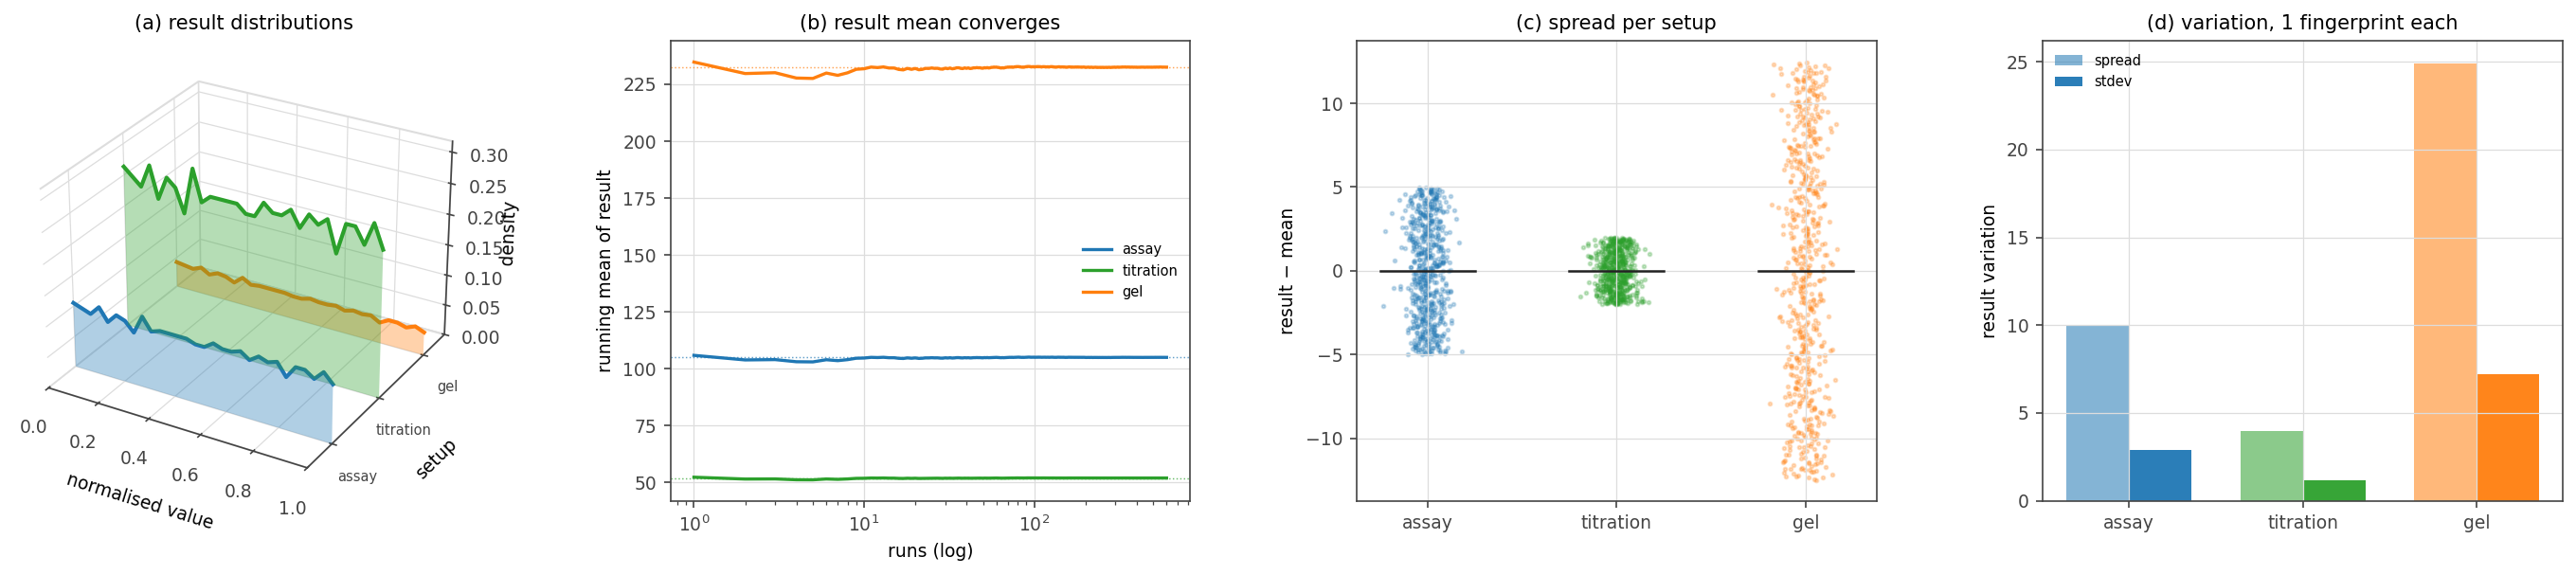
\includegraphics[width=\textwidth]{figures/panel_nondeterminism.png}
    \caption{\textbf{Reproducibility Attaches to the Protocol, Not the Results.}
    Executable model (\texttt{validation/nondeterminism\_provenance.py}): three
    imported standard setups---assay, titration, gel---each run $600$ times, the
    measurement outcome varying by a linear-congruential step while the structure
    is held fixed.
    (\textbf{A})~Three-dimensional ridgeline of result distributions, normalised
    value ($x$-axis, $0$ to $1$) against setup ($y$-axis: assay, titration, gel)
    against probability density ($z$-axis), viewing angle elevation $28^{\circ}$
    azimuth $-60^{\circ}$; each setup's histogram is drawn as a filled polygon in
    its own plane. Every setup spreads into a distribution rather than a spike.
    (\textbf{B})~Running mean of the result (linear $y$-axis) versus run index
    (log $x$-axis, $1$ to $600$), one line per setup with its limit as a dotted
    reference. The three means converge to distinct, stable levels---assay
    $105.007$, titration $52.003$, gel $232.517$---so the result varies run to run
    but its law is fixed by the protocol. Empirical content of
    Proposition~\ref{prop:nondeterminism} (Intended Non-Determinism).
    (\textbf{C})~Centred raw results (linear $y$-axis, result $-$ mean) as a jittered
    scatter over the three setups ($x$-axis), $600$ points each, with a black
    zero reference. The per-setup spread is manifestly different---full spans of
    $9.970$ (assay), $3.988$ (titration), and $24.925$ (gel) units---and is data,
    not defect.
    (\textbf{D})~Result variation by setup: paired bars of full spread (light) and
    standard deviation (dark), coloured per setup---spreads $9.970/3.988/24.925$,
    standard deviations $2.883/1.153/7.208$. Despite this variation each setup
    carries exactly \emph{one} provenance fingerprint across all $600$ runs
    (assay \texttt{f973f036}, titration \texttt{0880dc84}, gel \texttt{b5b72e72}),
    and the three fingerprints are distinct: the invariance of the fingerprint, not
    the coincidence of the numbers, is what reproducibility means here.}
    \label{fig:panel-nondeterminism}
\end{figure*}

% ---------------------------------------------------------------------------
% Panel 4: resolution / blast radius  (Def. resolution, Prop. prefix)
% ---------------------------------------------------------------------------
\begin{figure*}[!htbp]
    \centering
    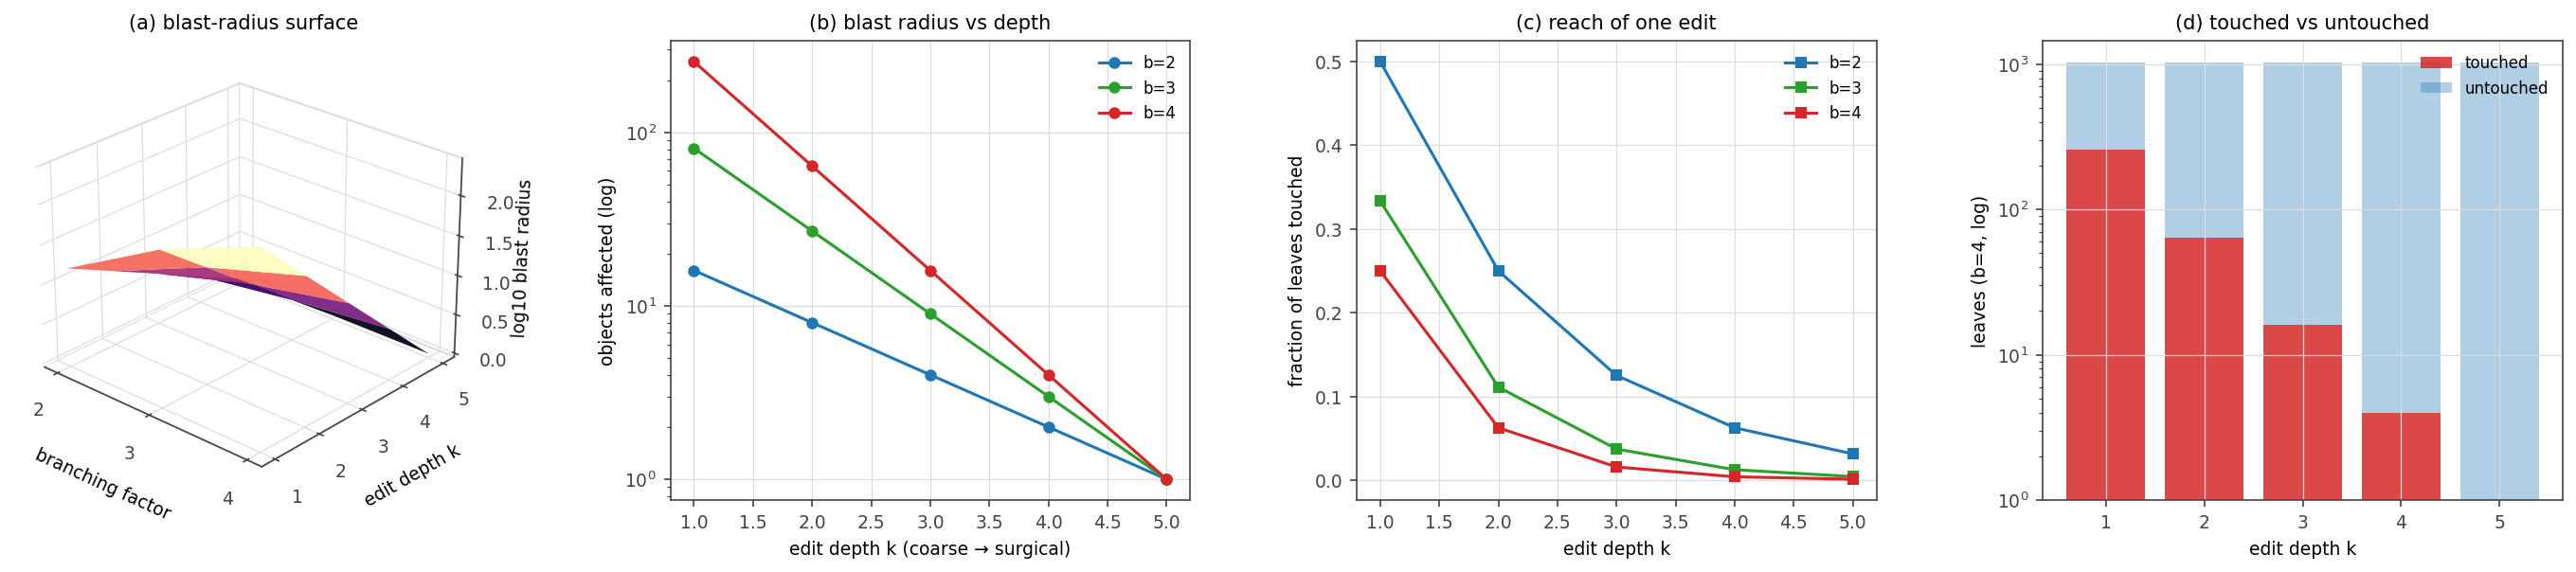
\includegraphics[width=\textwidth]{figures/panel_resolution.png}
    \caption{\textbf{One Computation at Any Resolution: Blast Radius $b^{\,D-k}$.}
    Executable model (\texttt{validation/resolution\_control.py}) over uniform
    address trees of branching factor $b \in \{2,3,4\}$ and depth $D=5$, editing a
    single address prefix at each depth $k$ and counting the leaf objects affected.
    (\textbf{A})~Three-dimensional magma surface of the blast radius on a
    $\log_{10}$ $z$-axis over branching factor ($x$-axis, $2$ to $4$) and edit
    depth $k$ ($y$-axis, $1$ to $5$), viewing angle elevation $26^{\circ}$ azimuth
    $-48^{\circ}$. The surface falls smoothly from a coarse edit's broad reach to a
    surgical edit's single leaf.
    (\textbf{B})~Objects affected on a log $y$-axis versus edit depth $k$ (linear
    $x$-axis, $1$ to $5$, coarse to surgical), one line per branching factor. The
    measured blast radii---$b\!=\!2\!:\,16,8,4,2,1$; $b\!=\!3\!:\,81,27,9,3,1$;
    $b\!=\!4\!:\,256,64,16,4,1$---coincide with the prediction $b^{\,D-k}$ to the
    leaf at every point. Empirical content of Proposition~\ref{prop:prefix}
    (Prefix Containment): editing at depth $k$ touches exactly the length-$k$
    prefix subtree.
    (\textbf{C})~The same as a fraction of the tree (linear $y$-axis) versus edit
    depth ($x$-axis), one line per branching factor. One edit's reach falls from
    the entire subtree at $k=1$ toward a vanishing fraction---a single leaf---at
    $k=D$, realising Definition~\ref{def:resolution} (Resolution): coarse and
    surgical control are one address space traversed to different depths.
    (\textbf{D})~Touched versus untouched leaves for the largest tree ($b=4$,
    $4^{5}=1024$ leaves) as stacked bars on a log $y$-axis over edit depth
    ($x$-axis, $1$ to $5$): touched leaves (red) fall $256 \to 64 \to 16 \to 4
    \to 1$ while the untouched remainder (blue) is byte-identical between runs.
    Control ranges from an entire imported region down to a single step, exercised
    only where the user reaches.}
    \label{fig:panel-resolution}
\end{figure*}

% ---------------------------------------------------------------------------
% Panel 5: cross-cutting synthesis
% ---------------------------------------------------------------------------
\begin{figure*}[!htbp]
    \centering
    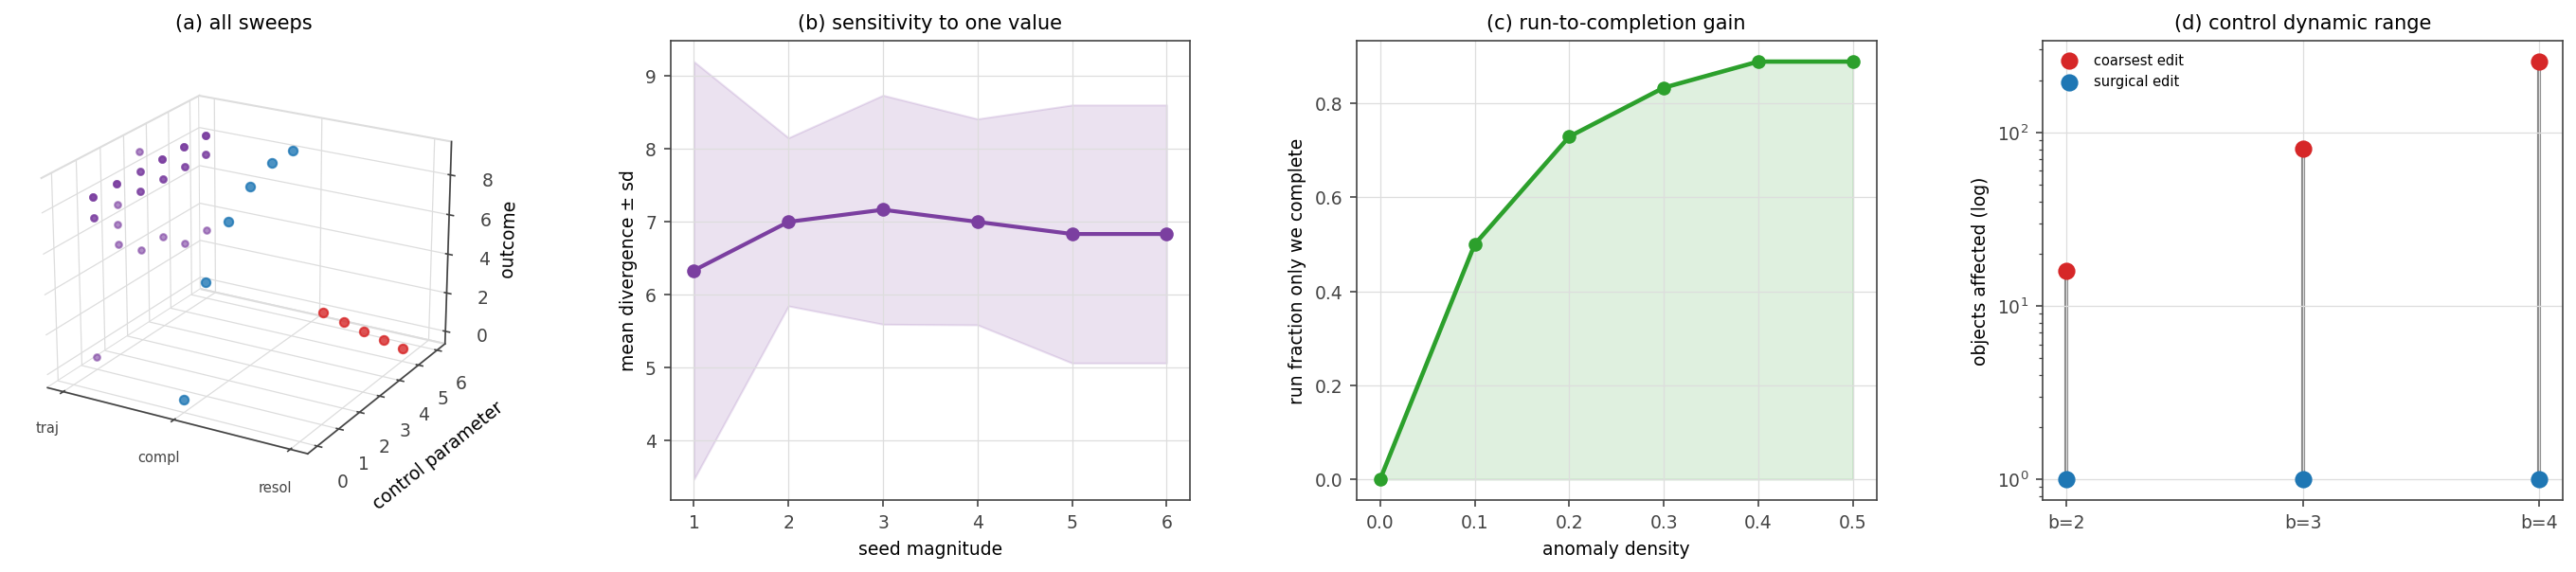
\includegraphics[width=\textwidth]{figures/panel_overview.png}
    \caption{\textbf{Cross Cutting Synthesis of the Runtime's Procedural Refusals and Affordance.}
    (\textbf{A})~Three-dimensional scatter placing every sweep run by claim family
    ($x$-axis: trajectory, completion, resolution), control parameter ($y$-axis),
    and outcome ($z$-axis), viewing angle elevation $22^{\circ}$ azimuth
    $-60^{\circ}$: the trajectory cloud (purple), completion-loss points (blue),
    and blast-radius points (red) occupy one figure, each claim a distinct
    signature in the outcome axis.
    (\textbf{B})~Mean trajectory divergence (linear $y$-axis) versus seed magnitude
    (linear $x$-axis, $1$ to $6$), collapsed over the six seeded nodes with a
    $\pm$ one-standard-deviation band: a single value's leverage on the induced
    edge relation, rising then levelling near seven edges of divergence.
    (\textbf{C})~Run-to-completion gain (linear $y$-axis)---the fraction of the run
    this runtime completes that a halt-on-error runtime abandons---versus anomaly
    density (linear $x$-axis, $0.0$ to $0.5$), green curve with shaded fill rising
    from $0$ to $0.89$: the advantage is largest exactly where anomalies are
    densest.
    (\textbf{D})~Dynamic range of resolution control: for each branching factor
    ($x$-axis, $b=2,3,4$) a vertical span on a log $y$-axis from the surgical edit
    ($1$ leaf, blue) to the coarsest edit ($16$, $81$, and $256$ leaves
    respectively, red). Together the panels present the runtime's three procedural
    refusals---no schedule, no exit code, no identical results---and its single
    affordance, absolute control at any resolution, as measured quantities rather
    than assertions.}
    \label{fig:panel-overview}
\end{figure*}
